\documentclass[xcolor=dvipsnames,aspectratio=169]{beamer}

\usepackage{fontspec}
\defaultfontfeatures{Ligatures=TeX}
%\setsansfont{Liberation Sans}
\usepackage{polyglossia}
\setdefaultlanguage{german}

\usetheme{Berlin}
\usecolortheme[named=LimeGreen]{structure}
\usepackage{beamerthemesplit} % kam neu dazu
			
\usepackage{amsmath}
\usepackage{graphicx}
\graphicspath{{pictures/}}
\usepackage{amssymb}
\usepackage{amsfonts}
\usepackage{caption}
\usepackage{multimedia}
\usepackage{tikz}
\usepackage{listings}
\usepackage{acronym}
\usepackage{lmodern}
\usepackage{multicol}
\usepackage{menukeys}

\definecolor{pblue}{rgb}{0.13,0.13,1}
\definecolor{pgreen}{rgb}{0,0.5,0}
\definecolor{pred}{rgb}{0.9,0,0}
\definecolor{pgrey}{rgb}{0.46,0.45,0.48}

\lstset{
    escapeinside={(*}{*)}
}

\lstdefinestyle{Java}{
  showspaces=false,
  showtabs=false,
  tabsize=2,
  breaklines=true,
  showstringspaces=false,
  breakatwhitespace=true,
  commentstyle=\color{pgreen},
  keywordstyle=\color{pblue},
  stringstyle=\color{pred},
  basicstyle=\footnotesize\ttfamily,
  numbers=left,
  numberstyle=\tiny\color{gray}\ttfamily,
  numbersep=7pt,
  %moredelim=[il][\textcolor{pgrey}]{$$},
  moredelim=[is][\textcolor{pgrey}]{\%\%}{\%\%},
  captionpos=b
}

\lstdefinestyle{basic}{  
  basicstyle=\footnotesize\ttfamily,
  breaklines=true
  numbers=left,
  numberstyle=\tiny\color{gray}\ttfamily,
  numbersep=7pt,
  backgroundcolor=\color{white},
  showspaces=false,
  showstringspaces=false,
  showtabs=false,
  frame=single,
  rulecolor=\color{black},
  captionpos=b,
  keywordstyle=\color{blue}\bf,
  commentstyle=\color{gray},
  stringstyle=\color{green},
  keywordstyle={[2]\color{red}\bf},
}


\lstdefinelanguage{custom}
{
morekeywords={public, void},
sensitive=false,
morecomment=[l]{//},
morecomment=[s]{/*}{*/},
morestring=[b]",
}


\lstdefinestyle{BashInputStyle}{
  language=bash,
  showstringspaces=false,
  basicstyle=\small\sffamily,
  numbers=left,
  numberstyle=\tiny,
  numbersep=5pt,
  frame=trlb,
  columns=fullflexible,
  backgroundcolor=\color{gray!20},
  linewidth=0.9\linewidth,
  xleftmargin=0.1\linewidth
}

\lstdefinestyle{Bash}{
  language=bash,
  showstringspaces=false,
  basicstyle=\small\sffamily,
  numbers=left,
  numberstyle=\tiny,
  numbersep=5pt,
  frame=trlb,
  columns=fullflexible,
  backgroundcolor=\color{gray!20},
  linewidth=0.9\linewidth,
  %xleftmargin=0.5\linewidth
}

%Logo in the upper right just change if you know what you are doing^^
\addtobeamertemplate{frametitle}{}{%
\begin{tikzpicture}[remember picture,overlay]
\node[anchor=north east,yshift=2pt] at (current page.north east) {
\includegraphics[height=1.8cm]{htw}};
\end{tikzpicture}}

\begin{document}
\bibliographystyle{alpha}
\title{Netzwerke und verteilte Systeme\\Übung\\Sommersemester 2021}
\subtitle{Grundlagen Unix \& Shell\\
\href{mailto:Benjamin.Troester@HTW-Berlin.de}{Benjamin.Troester@HTW-Berlin.de}\\
		PGP: ADE1 3997 3D5D B25D 3F8F 0A51 A03A 3A24 978D D673 }

\author{Benjamin Tröster}

\date{}

\begin{frame}
\titlepage
\end{frame}

\begin{frame}{Kurze Einführung zu Betriebssysteme}
 \vspace*{-0.8cm} 
	\begin{itemize}
		\item Wir arbeiten das Semester hauptsächlich mit Unix -- \emph{freeBSD}
		\item Warum?
		\begin{enumerate}
			\item Einfaches, direktes Tooling via Kommandozeile
			\item Sehr gute Dokumentation!
			\item Weniger schlecht Umgesetzt als Windows, Linux etc.
			\item Komplexe Abhängigkeiten eher die Ausnahme
			\item Keine Bevormundung: Wir entscheiden, was und wie das System arbeitet.
		\end{enumerate}
		\item Kurze Einführung zu den Themen
		\begin{itemize}
			\item Betriebssysteme
			\item Shell
		\end{itemize}
		\item Nächstes Semester eigene LV: Betriebssysteme
		\begin{itemize}
			\item Aufbau/Design von Betriebssystemen
			\item Basisfunktionalitäten \& -konzepte
			\item Programmierung von: Shell- \& Python-Skripten, C-Systemprogrammierung
		\end{itemize}
	\end{itemize}
\end{frame}

\section*{Road-Map}
\begin{frame}
\frametitle{Road-Map}
\begin{multicols}{2}
  \tableofcontents
\end{multicols}
\end{frame}
\section{Historisches zu Unix}
\begin{frame}
	\frametitle{Historisches zu Unix}
 \begin{tabular}{cc}
 \hspace*{-1.3cm} 
 \parbox{0.65\linewidth}{
\begin{itemize}
	\item Eigentlich von \ac{unics} -- Anspielung auf Multics \footnote{\url{https://de.wikipedia.org/wiki/Multics}}
	\item 1969 entwickelt in den Bell Laboratories
	\item Bekannte Vertreter:
	\begin{itemize}
	\item \ac{bsd}, SunOS/ Solaris, Minix, OpenBSD, IllumOS, FreeBSD
	\item \url{https://de.wikipedia.org/wiki/Berkeley_Software_Distribution}
	\end{itemize}
\end{itemize} } 
& \begin{tabular}{l}
 \begin{tabular}{c}
 \hspace*{-1.1cm}
           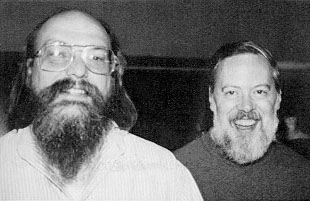
\includegraphics[scale=0.65]{Ken_n_dennis}
           \end{tabular}
\end{tabular}\\
\end{tabular}
\end{frame}

\begin{frame}
\begin{figure}
\centering
 \vspace*{-.2
 cm} 
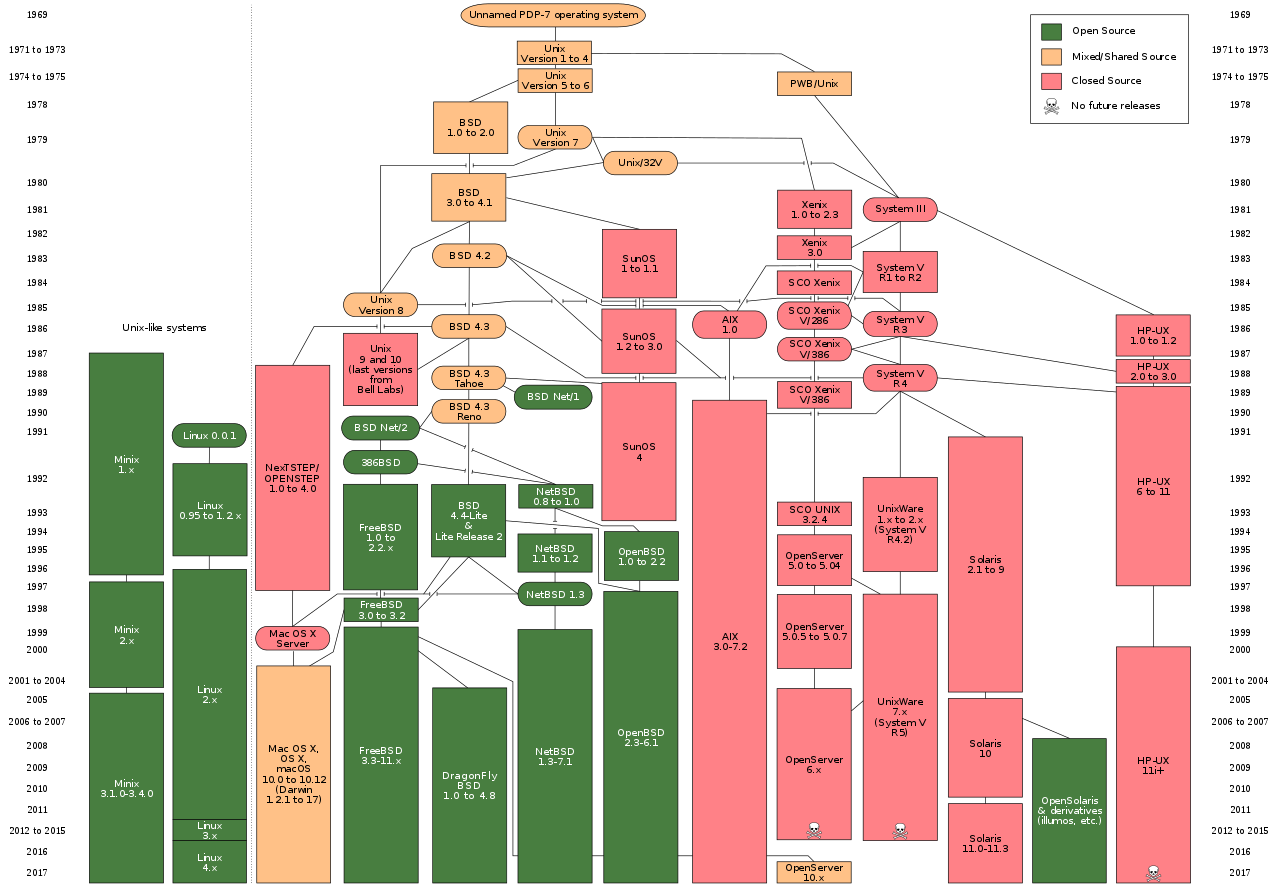
\includegraphics[scale=0.18]{unix_hist}
\caption{Zeitliche Einordnung der Unix-Historie. (s. \url{https://en.wikipedia.org/wiki/History_of_Unix}) }
\end{figure}
\end{frame}

\subsection{Linux}
\begin{frame}{Linux}
\begin{tabular}{lc}
\hspace{-1.3cm}
 \parbox{0.65\linewidth}{
 \vspace{-0.25cm}
\begin{itemize}
	\item 1991 im Usenet \footnote{\url{https://de.wikipedia.org/wiki/Usenet}} veröffentlicht von Linus Torvalds
	\item Linux im wesentlichen Kernel (Betriebssystemkern) + GNU-Tools (Compiler, Debugger etc.)
	\begin{itemize}
		\item Kernel übernimmt die elementarsten Aufgaben im BS (s. \url{https://en.wikipedia.org/wiki/Kernel_(operating_system)})
	\end{itemize}
	\item Distributionen nutzen (angepassten) Linux Kernel + (eigene) Standardsoftware -- Paketmanager etc.
	\item Bekannte Linux Distributionen:
	\begin{itemize}
	\item Slackware, Red Hat, Debian, Gentoo, Arch
	\item Mehr unter: \url{https://www.kernel.org/}
	\end{itemize}
\end{itemize} } 
& \begin{tabular}{c}
 \hspace{1.5cm}
           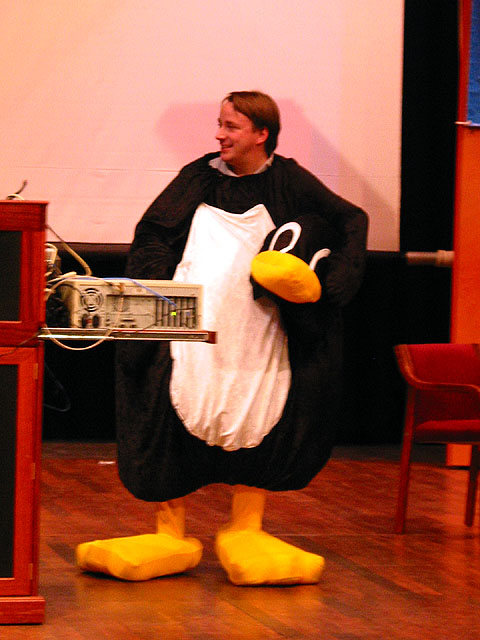
\includegraphics[scale=0.215]{linus}
           \end{tabular}
\end{tabular}
\end{frame}

\section{Unixoide Betriebssysteme}
\subsection{Aufgaben des OS'}

\begin{frame}{}
  \tableofcontents[currentsection,hideothersubsections]
\end{frame}

\begin{frame}
	\frametitle{Hauptaufgaben des Betriebssystems}
	\begin{itemize}
		\item Bereitstellen einer virtuellen Maschine \url{https://de.wikipedia.org/wiki/Virtuelle_Maschine}
		\begin{itemize}
			\item als Abstraktion des Rechnersystems
		\end{itemize}
		\item Verwaltung und Operationen auf den Ressourcen
		\begin{itemize}
			\item physische Ressourcen
			\item logische Ressourcen
		\end{itemize}
		\item Adaption der Rechnerstruktur für Nutzeranforderungen
		\item Legt die Grundlage für geregelten, nebenläufigen Ablauf der Aktivitäten
		\item Verwaltung der Daten \& Ressourcen
		\item Unterstützung bei Fehlern \& Ausfällen ...
	\end{itemize}
\end{frame}

\subsection{Architektur (monolithischer Kernel)}
\begin{frame}{Aufbau eines Betriebssystems: Ringmodell}
	\vspace{-.7cm}
 \begin{tabular}{cc} 
 \hspace*{-1.3cm} 
 \parbox{0.65\linewidth}{
\begin{itemize}
	\item Hardware
	\begin{itemize}
		\item CPU, RAM, Mainboard ...
	\end{itemize}
	\item Kernel -- Betriebssystemkern
	\begin{itemize}
		\item Prozessteuerung, Systemaufrufe, (Gerätetreiber, Dateisystem) ...
	\end{itemize}
	\item Shell -- Schnittstelle zwischen Nutzer \& Diensten des Betriebssystems
	\begin{itemize}
		\item \ac{cli} oder \ac{gui}
		\item Interpretiert \& bearbeitet Eingaben des Nutzers
	\end{itemize}
	\item Anwendungsprogramme
	\begin{itemize}
		\item Standardsoftware \& 3rd-Party-Software
	\end{itemize}

\end{itemize} } 
& \begin{tabular}{l}
 \begin{tabular}{c}
 \vspace{-.05cm}
 %\hspace*{-.5cm}
           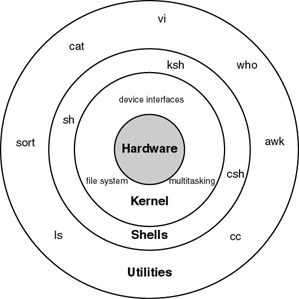
\includegraphics[scale=0.5]{unix_arch}
           \end{tabular}
\end{tabular}\\
\end{tabular}
\end{frame}


\subsection{Dateisysteme}
\begin{frame}{Dateisysteme}
	\begin{itemize}
		\item Dateisystem ist die Abstraktion der eigentlichen physischen Ressource (HDDs, SSDs,...)
		\item Dateien sind logische Ressourcen $\rightarrow$ Kollektion von logischen Dateneinheiten -- Records
		\item Dateisysteme richten sich (wie Betriebssysteme) nach den Systemanforderungen
		\item Beispiele:
		\begin{itemize}
			\item FAT -- File Allocation Table
			\item NTFS -- New Technology File System
			\item UFS -- Unix File System
			\item ZFS -- Zettabyte File System
		\end{itemize}
	\end{itemize}
\end{frame}

\begin{frame}{Bäume}
\begin{tabular}{lc}
\hspace{-1.3cm}
 \parbox{0.65\linewidth}{
 \vspace{-0.25cm}
	\begin{itemize}
	\item Mathematische Struktur -- spezieller, zusammenhängender, azyklischer Graph (Graphentheoreie)
	\item In Unix-Dateisystem: Es gibt ein Wurzelelement:\\ "\path{/}" -- sprich: \emph{root}
	\item Alle anderen Einträge (Ordner, Dateien etc.) sind dem Wurzelelement untergeordnet
\end{itemize} } 
& \begin{tabular}{c}
 \hspace{1.5cm}
           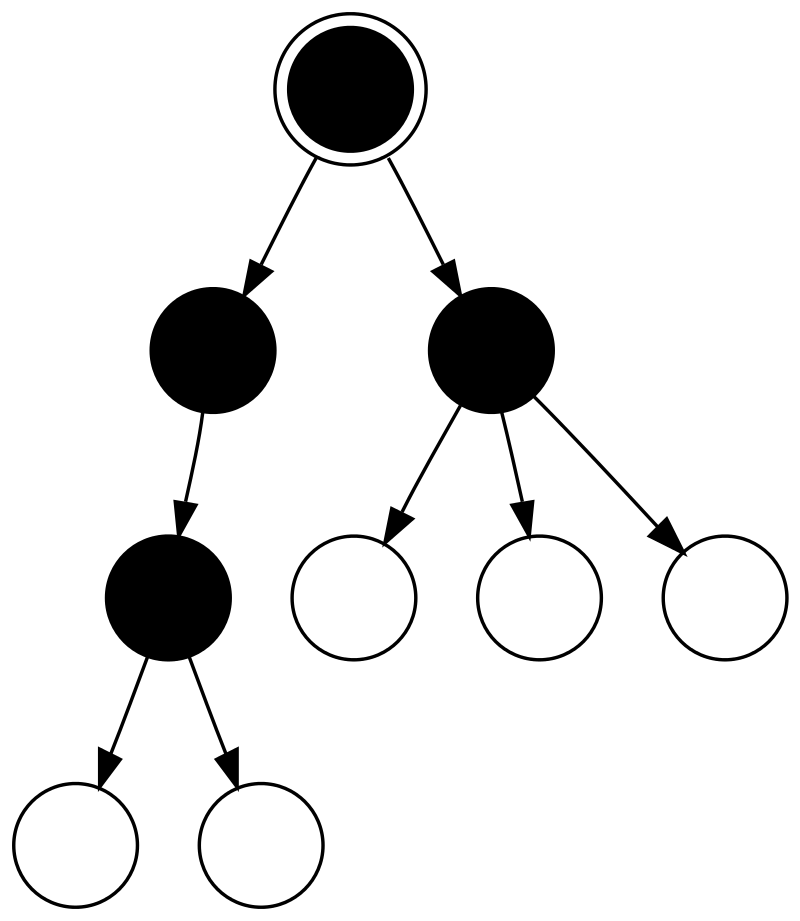
\includegraphics[scale=0.1]{Directed-tree}
           \end{tabular}
\end{tabular}
\end{frame}

\begin{frame}
\begin{figure}
  \vspace*{-0.17cm}
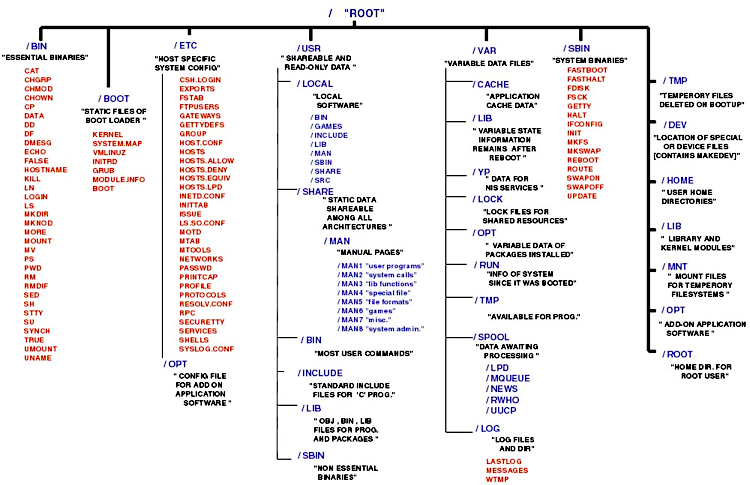
\includegraphics[scale=0.4]{filesystem}
\end{figure}
\end{frame}

\begin{frame}{Dateisystem cnt.}
\vspace{-.5cm}
In Linux/Unix ist grundsätzlich alles eine Datei!\\
\textbf{Baumstruktur -- statt separate Massenspeicher}\\
Exemplarisch:
\begin{itemize}
	\item / -- Wurzelverzeichnis
	\item /bin -- wichtigste Programme in Binäreformat
	\item /boot -- Boot-Loader
	\item /etc -- System Konfiguration
	\begin{itemize}
		\item /usr/local -- lokale Software
		\item /usr/bin -- User-Land-Software
		\item /usr/include -- Standard-Bibliotheken für C/C++
		\item /usr/lib -- Bibliotheken für Programmiersprachen
	\end{itemize}
	\item ...
\end{itemize}
\end{frame}


\subsection{User \& Gruppen}
\begin{frame}
Linux/Unix sind Mehrbenutzersysteme, d.h. mehrere Nutzer können simultan auf einem Rechner arbeiten
\begin{itemize}
	\item Zuordnung der Nutzer zu User \& Group
	\item Regelt Zugangskontrolle im System auf
	\begin{itemize}
	\item  Dateien, Ordner \& Peripheriegeräte
	\end{itemize}
	\item Unterschiedliche Nutzer/Gruppen $\rightarrow$ unterschiedliche Rechte
	\item Im Labor:
	\begin{itemize}
		\item Benutzername: Matrikelnummer
		\item Gruppen: student, domain, users,...
	\end{itemize}
	\item Virtual Machine (Debian):
	\begin{itemize}
		\item Benutzername: student
		\item Gruppen: student, users, wireshark,...
	\end{itemize}
\end{itemize}
\end{frame}

\subsection{Ziffer- und Positionssysteme}
\begin{frame}{Ziffer- und Positionssysteme}
\vspace{-0.5cm}
\begin{itemize}
	\item Dezimalsystem -- Basis 10
	\begin{itemize}
		\item Werte 0 - 9 
		\item Beispiel: $42_{10}$
	\end{itemize}
	\item Dualsystem/ Binärsystem -- Basis 2
	\begin{itemize}
		\item Werte 0 oder 1
		\item Bit-Darstellung in der Informatik/ Rechnertechnik
		\item Beispiel: $42_{10} = 0010~1010_2$
	\end{itemize}
	\item Oktalsystem -- Basis 8
	\begin{itemize}
		\item Werte 0 - 7
		\item Für Darstellung der Zahlen 0 - 7 $\rightarrow$ 3 Bit notwendig, $2^3 = 8$
		\item Beispiel: $42_{10} = 52_8 = 0010~1010_2$
	\end{itemize}
	\item Sehr schöne Aufarbeitung, Kapitel 1.1.2ff: \url{http://numerik.mi.fu-berlin.de/matheon-G8/comaBuch.pdf}
\end{itemize}
\end{frame}

\subsection{DAC}
\begin{frame}{Discretionary Access Control}
Zugriff auf Dateien allein anhand der Identität.\\
Ressourcenzugriff haben Eigentümer \& Gruppe -- regeln Abbildung auf Nutzer
\begin{itemize}
	\item Grundsätzlich in drei Kategorien:
	\begin{itemize}
		\item Owner -- regelt Berechtigung des Eigentümers
		\item Group -- regelt Berechtigung der Gruppe
		\item Other (world) -- regelt Berechtigung aller anderen Nutzer 
	\end{itemize}
	\item Unix Zugriffsmodi:
	\begin{itemize}
		\item read (r) -- Lesezugriff
		\item write (w) -- Schreibzugriff
		\item execute (x) -- Ausführzugriff
	\end{itemize}
\end{itemize}
\end{frame}

\begin{frame}{Discretionary Access Control}
Darstellung im System via Oktalzahlen:
\begin{itemize}
	\item Zuordnung der Berechtigung r,w,x bestimmten Werten
	\begin{itemize}
		\item Lesen (r) $\rightarrow$ $4_8$ oder $100_2$
		\item Schreiben (w) $\rightarrow$ $2_8$ oder $010_2$
		\item Ausführen (x) $\rightarrow$ $1_8$ oder $001_2$
		\item None $\rightarrow$ $0_8$ oder $000_2$
	\end{itemize}
	\item Zusammensetzen der Oktalwerte ergibt Zugriffsrechte:
	\begin{itemize}
		\item Lesen, schreiben und ausführen $\rightarrow$ $7_8$ oder $111_2$
		\item Lesen und Schreiben $\rightarrow$ $6_8$ oder $110_2$
		\item Lesen und Ausführen $\rightarrow$ $5_8$ oder $101_2$
		\item ...
	\end{itemize}
\end{itemize}
\end{frame}

\begin{frame}{Discretionary Access Control}
Zusammensetzung der Berechtigung
\begin{itemize}
	\item 3er-Oktett gibt Zugriffsmodalitäten an
	\begin{enumerate}
		\item user r,w,x -- erstes Oktett
		\item group r,w,x -- zweites Oktett
		\item other r,w,x -- drittes Oktett
	\end{enumerate}
\end{itemize}
\begin{figure}
	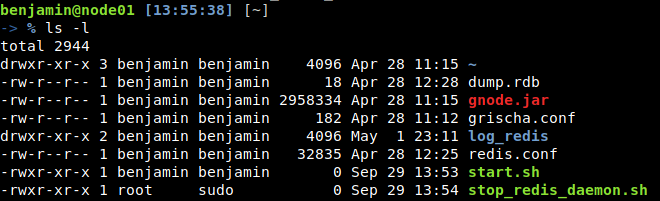
\includegraphics[scale=0.5]{rights}
\end{figure}
\end{frame}

\section{Systemcalls \& Daemons}
\begin{frame}{Systemcalls \& Daemons -- !Short Version}
	\begin{itemize}
		\item Systemcalls -- Methode für Anwendungsprogramme, um Funktionalitäten des BS' nutzen zu können
		\item Systemcalls vollführen Wechsel von Anwenderebene auf BS-Kern 
		\item Übergabe der Kontrolle von Anwender an das Betriebssystem
		\begin{itemize}
			\item Bspw.: anlegen von Dateien auf SSD, Verbindung des Browsers zu einer Webseite etc.
		\end{itemize}
		\item Daemons -- Hintergrunddienste
		\item Stellen Dienste des BS bereit, auf die Programme zugreifen können
		\begin{itemize}
			\item Bsp: Netzwerkdienste, Sockets ...
		\end{itemize} 
	\end{itemize}
\end{frame}

\section{Unix-Philosophie}

\begin{frame}{}
  \tableofcontents[currentsection,hideothersubsections]
\end{frame}

\begin{frame}{Unix-Philosophie}
	Nach Douglas McIlroy \footnote{\url{https://en.wikipedia.org/wiki/Douglas_McIlroy}} \footnote{\url{https://homepage.cs.uri.edu/~thenry/resources/unix_art/ch01s06.html}}
	\begin{itemize}
		\item Schreibe Computerprogramme so, dass sie nur eine Aufgabe erledigen und diese gut machen.
		\item Schreibe Programme so, dass sie zusammenarbeiten.
		\item Schreibe Programme so, dass sie Textströme verarbeiten, denn das ist eine universelle Schnittstelle.
	\end{itemize}
	\textbf{Bottom-Line:} Baue Programme derart das Interoperabilität besteht, sodass komplexere Probleme lösbar sind!
\end{frame}

\section{Shell}

\begin{frame}{}
  \tableofcontents[currentsection,hideothersubsections]
\end{frame}

\subsection{Einführung}
\begin{frame}{Einführung Shell}
	\begin{itemize}
		\item Textbasierte Schnittstelle
		\item Schnittstelle zwischen BS-Kern, Werkzeugen des BS' \& User
		\item Shell ist ein Kommando-Interpreter $\rightarrow$ führt Schrittweise Befehle aus
		\begin{itemize}
			\item Kommandos sind oft Binärdateien, Programmskripte
			\item Kommandos können direkt aufgerufen werden
			\item Aufruf von Systemcalls möglich $\rightarrow$ Administration des Systems
		\end{itemize}
	\end{itemize}
\end{frame}

\begin{frame}{Shells}
	\begin{itemize}
		\item Ur-Shell: Thompson Shell -- OSH
		\item SH -- Bourne Shell 
		\item BASH -- Bourne Again Shell
		\item CSH -- C Shell
		\item TCSH -- TENEX C Shell
		\item KSH -- Korn Shell
		\item ZSH -- Zhong Shao Shell
		\item ...
	\end{itemize}
\end{frame}

\subsection{Shell 101}
\begin{frame}{Shell 101}
	\begin{itemize}
		\item In der VM: \keys{\winmenu} (Windowstaste) und dann einfach Terminal eingeben
		\item Alternativ: \keys{\ctrl + \Alt + t} (Str + Alt + t)
		\item Abbrechen eines Kommandos: \keys{\ctrl + c} (Str + c)
		\item Beenden/Schließen des Terminals: \keys{\ctrl + d} (Str + d) oder einfach \emph{exit} eintippen
	\end{itemize}
\end{frame}

\subsection{Shell Input/Output}
\begin{frame}{Shell Input/Output}
	\begin{itemize}
		\item Kommandozeile hat drei Standardkanäle:
		\begin{enumerate}
			\item Standardinput (stdin) -- Eingabe von Daten
			\item Standardoutput (stdout) -- Ausgabe von Daten
			\item Standarderror (stderr) -- Ausgabekanal im Fall von Fehlern
		\end{enumerate}
		\item Ausgabe von Tools zumeist auf stdout
		\item Ein- \& Ausgabe kann jedoch auch umgelenkt werden
		\item Ausgabe kann somit in Datei geschrieben bzw. aus Datei gelesen werden
		\item Verbinden von Kommandos durch \emph{Piping}
		\begin{itemize}
			\item Ausgabe eines Programms wird Eingabe des anderen Programms
		\end{itemize}
		\item Schauen Sie sich die Links im Moodle-Kurs an!
	\end{itemize}
\end{frame}

\begin{frame}
	\frametitle{Input/Output Redirection}
\begin{itemize}
	\item Umlenken der Ausgabe in eine Datei: \keys{>}
		\begin{itemize}
			\item Lenkt Ausgabe in eine Datei
			\item Datei wird dabei vollständig neu geschrieben
			\item Alter Inhalt geht verloren
		\end{itemize}
	\item Anfügen einer Datei: \keys{> >}
	\begin{itemize}
		\item Hängt Ausgabe an das Ende der Datei 
	\end{itemize}
	\item Umlenken der Eingabe aus einer Datei: \keys{<}
		\begin{itemize}
			\item Programm erhält zeilenweise Eingabe aus der Ressource
		\end{itemize}
\end{itemize}
\end{frame}

\begin{frame}
	\frametitle{Piping}
\begin{itemize}
	\item Verbinden mehrerer Kommandos durch eine \emph{Pipe}
	\item Pipe: Datenstruktur -- Folgt dem First-In-First-Out-Prinzip (FIFO)
	\item Wirkt wie ein Puffer, eingehende Daten werde gepuffert und bei Bedarf wieder ausgegeben
	\item Piping ermöglicht es Programme zu verbinden
	\item Ausgabestrom eines Programm wird Eingabestrom des nächsten Programms
	\item \textbf{Vorteil:} Einfache Programme können zu mächtigeren Programmen zusammengesetzt werden
	\item Folgt der Unix-Philosophie
\end{itemize}
\end{frame}

\begin{frame}[fragile]{Beispiele}
	\begin{lstlisting}[style=Bash, language=Bash]
date > foo.txt
echo "student name" >> studi_list_1.csv
head < studi_list_1.csv
sort studi_list_1.csv studi_list_2.csv | uniq -u > clean_list.csv
	\end{lstlisting}
\end{frame}

\begin{acronym}
\acro{bsd}[BSD]{Berkeley Software Distribution}
\acro{cli}[CLI]{Command Line Interface}
\acro{dfn}[DFN]{Deutsches Forschungsnetz}
\acro{gui}[GUI]{Graphical User Interface}
\acro{gw}[GW]{Gateway}
\acroplural{gws}[GW`s]{Gateways}
\acro{lan}[LAN]{Local Area Network}
\acro{moco}[MOCO]{Mobile Computing}
\acro{soc}[SoC]{System on a chip}
\acro{wan}[WAN]{Wide Are Network}
\acro{unics}[UNICS]{Uniplexed Information and Computing Service}
\end{acronym}

\end{document}